%% SuperZero: project report on an AlphaZero-style agent for Ultimate Tic-Tac-Toe.
%% Kit: IEEEtran conference class (IEEEtran.cls / IEEEtran.bst copied up from CTAN V1.8b, never edited).
%% Build: pdflatex main && bibtex main && pdflatex main && pdflatex main
%% Figures: ../docs/report/figures, regenerated by scripts/report_figures.py and copied into figures/.
\documentclass[conference]{IEEEtran}
\IEEEoverridecommandlockouts
\usepackage{cite}
\usepackage{amsmath,amssymb,amsfonts}
\usepackage{graphicx}
\usepackage{textcomp}
\usepackage{xcolor}
\usepackage{booktabs}
\usepackage[protrusion=false]{microtype}
\usepackage{array}
\usepackage{adjustbox}
\usepackage{url}
\usepackage[hidelinks]{hyperref}
\graphicspath{{figures/}}
\renewcommand{\arraystretch}{0.95}

% Uniform float spacing
\setlength{\textfloatsep}{9pt plus 2pt minus 3pt}
\setlength{\dbltextfloatsep}{9pt plus 2pt minus 3pt}
\setlength{\floatsep}{7pt plus 2pt minus 2pt}
\setlength{\dblfloatsep}{7pt plus 2pt minus 2pt}
\setlength{\intextsep}{7pt plus 2pt minus 2pt}

% Notation macros: one command per defined name, never retyped
\newcommand{\code}[1]{\texttt{#1}}
\newcommand{\utttai}{uttt.ai}
\newcommand{\sys}{SuperZero}   % name of the agent / system
\newcommand{\net}{MMNet}       % name of the micro--macro network

\title{\sys: An AlphaZero-Style Agent for Ultimate Tic-Tac-Toe}
\author{\IEEEauthorblockN{Zamiul Rashid}}

\begin{document}
\maketitle

\begin{abstract}
This report describes \sys, a program that learns to play Ultimate
Tic-Tac-Toe. It follows the AlphaZero recipe: a neural network predicts which moves look
good and who is winning, Monte Carlo tree search uses those predictions to
look ahead, and the network is trained on the search's own results. The
network, \net, mirrors the game's two levels (a $9\times9$ grid of cells
and a $3\times3$ grid of boards); the training opponents are a mix of self-play,
classical alpha--beta search and two external engines, and a C++ bitboard
engine keeps the whole loop fast enough for a single workstation. We
explain the game, the method, the implementation, and the measured results.
The agent beats every classical baseline we built, including a depth-10
alpha--beta searcher with a 50-million-node cap (78.5\% over 72 games), and
the latest checkpoint (iteration 6000) finishes
first in a seven-engine round robin, ahead of the strongest public engine we
integrated, \utttai, with a 5--12--3 head-to-head record (55\%).
\end{abstract}

% ---------------------------------------------------------------------
\section{Introduction}

Ultimate Tic-Tac-Toe is Tic-Tac-Toe played on nine Tic-Tac-Toe boards at
once, with one twist: the cell you pick decides which board your opponent
must play in next. That twist links every local move to a global
consequence, and it makes the game hard enough that exhaustive analysis
only recently proved the first player's forced win (43 moves at best, while
the second player can hold out for at least 29 \cite{bertholon2020uttt}).

The project's goal was to build a strong player for this game, \sys,
using the AlphaZero approach \cite{silver2017alphazero} on a laptop-class
GPU rather than a data centre. This report explains what the game is, how
AlphaZero-style learning works, how our implementation is put together,
and what it achieved.

% ---------------------------------------------------------------------
\section{The Game}
\label{sec:game}

The board is a $3\times3$ grid of \emph{local boards}, each a $3\times3$
Tic-Tac-Toe board, for 81 cells. X and O alternate, X first.
\begin{itemize}\setlength{\itemsep}{0pt}
  \item A move marks an empty cell in an open local board.
  \item The \emph{position} of that cell inside its board decides which
        board the opponent must play in next: play the top-right cell of any
        board and the opponent is sent to the top-right board.
  \item If that board is already closed (won or full), the opponent may
        play anywhere (a \emph{free} move). The very first move is free.
  \item Three in a row wins a local board, which is then marked for that
        player on the \emph{macro board}; a full board with no line is
        drawn. Nothing more is played in a closed board.
  \item Three local wins in a row on the macro board wins the game; all
        nine boards closed with no macro line is a draw.
\end{itemize}
Forced moves have at most 9 options, free moves up to 81. In code, a state is $s=(C,B,t,f,r)$: the 81 cell
contents, the 9 board results, the player to move $t\in\{-1,+1\}$, the
forced board $f\in\{-1,0,\dots,8\}$ ($-1$ = free), and the result $r$ if the
game is over. An action is one integer $a=9b+c$ (board $b$, cell $c$), and
every agent in the system---neural, alpha--beta, external---uses this same
81-action interface.

% ---------------------------------------------------------------------
\section{How AlphaZero-Style Agents Work}
\label{sec:background}

AlphaGo, AlphaGo Zero and AlphaZero
\cite{silver2016alphago,silver2017alphagozero,silver2017alphazero} share
three ideas. Our system is a set of specific choices inside each.

\paragraph{Tree search guided by a prior.}
Classical programs search the game tree with minimax and alpha--beta
pruning \cite{knuth1975alphabeta}, cutting branches that cannot change the
answer and scoring the frontier with a hand-written heuristic. We keep
such a searcher as a baseline, but the learning agent uses Monte Carlo tree
search (MCTS), which grows a lopsided tree by repeating: \emph{select} a
path from the root, \emph{expand} a leaf, \emph{evaluate} it, \emph{back
up} the value. AlphaZero selects children with the PUCT rule
\cite{rosin2011puct}
\begin{equation}
  a^\ast=\arg\max_{a}\Bigl[\,Q(s,a)+c_{\mathrm{puct}}\,P(s,a)\frac{\sqrt{N(s)}}{1+N(s,a)}\Bigr],
  \label{eq:puct}
\end{equation}
where $Q$ is the average backed-up value of a child, $N$ counts visits,
and $P(s,a)$ is a learned \emph{prior} that says which moves deserve
attention. After a fixed number of \emph{simulations}, the root visit
counts $N(s,a)$ form an improved move distribution $\pi$, sharper than the
prior.

\paragraph{One network for policy and value.}
A network $f_\theta(s)=(\mathbf p,v)$ outputs the prior over moves and a
scalar $v\in[-1,1]$ estimating the result from the mover's point of view.
The prior concentrates a small search budget on plausible moves and the
value replaces the horizon heuristic, which is why 512 guided simulations
can compete with a brute-force search of tens of millions of nodes.

\paragraph{Self-play policy iteration.}
The agent plays itself using search. Every position is stored with the
search distribution $\pi$ and the eventual outcome $z\in\{-1,0,1\}$, and
the network is trained to imitate the search and predict the result,
$\mathcal L=-\pi^\top\log\mathbf p_\theta+(v_\theta-z)^2$. A better network
gives a better search, which gives better targets. AlphaZero starts from
random weights on thousands of TPUs; on one GPU we had to bootstrap from a
supervised dataset, mix in outside opponents, and add an extra training
signal, as described next.

% ---------------------------------------------------------------------
\begin{figure*}[t]
  \centering
  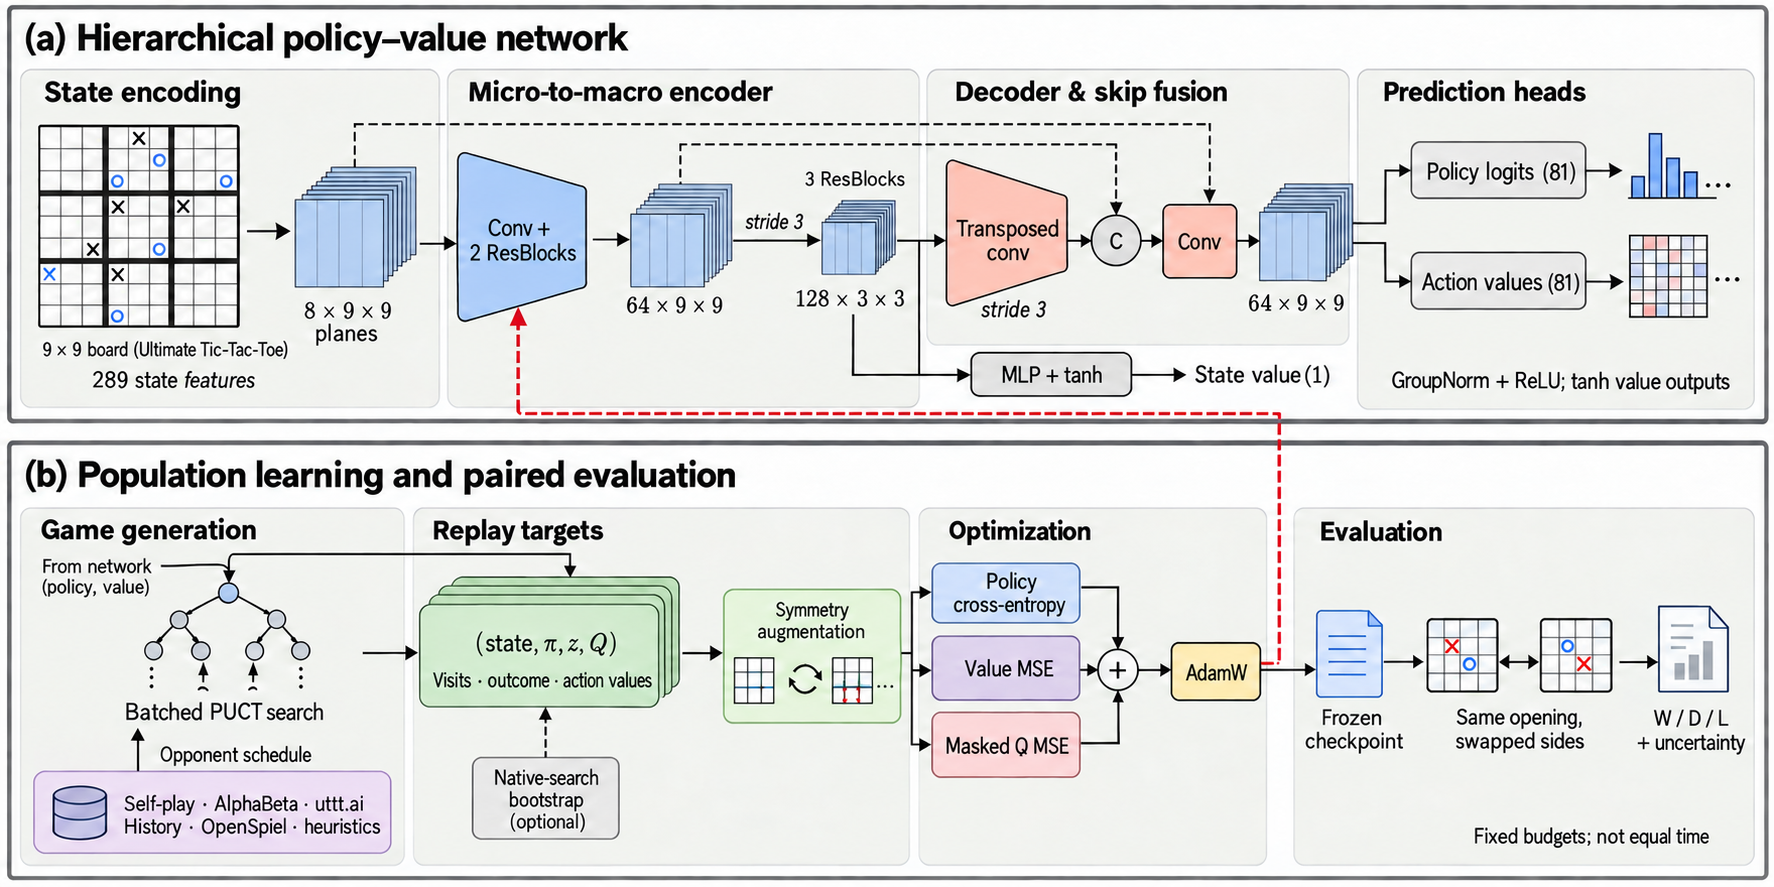
\includegraphics[width=\textwidth]{methodology.png}
  \caption{\sys\ overview. (a)~\net: eight $9\times9$ input
  planes $\to$ micro encoder $\to$ stride-3 pooling to a $3\times3$ macro
  grid $\to$ residual blocks $\to$ stride-3 upsampling $\to$ fusion with
  the micro features and input planes $\to$ policy and action-value heads;
  the state-value head reads the macro features. (b)~Training: batched
  PUCT search against a scheduled opponent population produces
  $(s,\pi,z,Q)$ rows that are symmetry-augmented and optimised with the
  three-term loss; frozen checkpoints are evaluated with mirrored seats.}
  \label{fig:overview}
\end{figure*}

\section{Our System}
\label{sec:system}

\subsection{Encoding and network}

A position is encoded relative to the player to move as 289 floats:
three one-hot cell planes (empty/mine/theirs, 81 each), four one-hot board
planes (open/mine/theirs/drawn, 9 each) and a 10-way one-hot for the forced
board. Inside the network this vector is reshaped into eight $9\times9$
planes in true grid order, so neighbouring cells are neighbouring pixels.

The first network was a flat residual MLP (\code{Linear(289,512)}, three
residual blocks) that treated the 81 cells as unrelated coordinates. It
was replaced by \net\ (Table~\ref{tab:unet}, Fig.~\ref{fig:overview}a),
a hierarchical network modelled on the \utttai\ architecture
\cite{waczynski2021utttai}: convolutions on the $9\times9$ cell grid, a
stride-3 convolution that pools each local board into one cell of a
$3\times3$ macro grid, residual blocks on the macro grid, a stride-3
transposed convolution back to $9\times9$, and U-Net-style skip
connections \cite{ronneberger2015unet}. The two resolutions are exactly the
game's two levels. The state value is read from the macro features
(``who is winning'' is a macro-board question); the policy and the
per-move action values are read from the fused cell features. GroupNorm
\cite{wu2018groupnorm} replaces BatchNorm because one module serves both
search batches (1--64 positions) and training batches (512--1024). \net\ has 1{,}560{,}835 parameters.

\begin{table}[t]
  \centering\footnotesize
  \caption{\net\ configuration (\code{sttt/unet.py}); shapes omit batch.}
  \label{tab:unet}
  \begin{tabular}{@{}lll@{}}
    \toprule
    Stage & Operation & Output \\
    \midrule
    Input & reshape/broadcast encoding & $8\times9\times9$ \\
    Stem & $3\times3$ conv, GroupNorm, ReLU & $64\times9\times9$ \\
    Micro & $2\times$ residual conv block & $64\times9\times9$ \\
    Pool & $3\times3$ conv, stride 3 & $128\times3\times3$ \\
    Macro & $3\times$ residual conv block & $128\times3\times3$ \\
    Up & $3\times3$ transposed conv, stride 3 & $64\times9\times9$ \\
    Fuse & concat[micro, up, input]; $3\times3$ conv & $64\times9\times9$ \\
    Policy & $1\times1$ conv & 81 logits \\
    Q head & $1\times1$ conv, $\tanh$ & 81 values \\
    Value & flatten macro; MLP $1152{\to}256{\to}1$, $\tanh$ & 1 \\
    \bottomrule
  \end{tabular}
\end{table}

\subsection{Search}

The search is PUCT (Eq.~\ref{eq:puct}) with $c_{\mathrm{puct}}=1.5$ and
Dirichlet root noise ($\alpha=0.3$, 25\% mix), plus four additions that
exist identically in the Python reference and the C++ engine:
\begin{itemize}\setlength{\itemsep}{0pt}
  \item \textbf{Batched evaluation.} Up to $L$ leaves (64 in training, 16
        in evaluation) are collected and sent to the network in one call.
        While a leaf is pending, its path carries a \emph{virtual loss} so
        that the next selection explores elsewhere.
  \item \textbf{Proofs.} Terminal values are exact, a node whose children
        are all proven is itself proven, and proven values are never
        overwritten by network estimates. A proven root stops early.
  \item \textbf{Soft pruning.} After 8 visits, a child whose $Q$ trails
        the best by more than 0.2 gets a reduced exploration weight (never
        below 0.2), and every 64th selection revisits the neglected child.
  \item \textbf{Subtree reuse.} The chosen child's subtree becomes the
        next root.
\end{itemize}
After each search, the mean value $q_a=W(s,a)/N(s,a)$ of every visited
root child is recorded along with a mask of which moves were visited.

\subsection{Training targets and loss}

Each stored position carries the encoding $x$, the visit distribution
$\pi$, the legal mask, the game outcome $z$ from the mover's view, and the
root action values $q$ with their visited mask $m^Q$. The loss is the
AlphaZero objective plus a masked action-value regression taken from
\utttai:
\begin{equation}
\begin{split}
  \mathcal L={}&\underbrace{-\!\!\sum_{a\ \mathrm{legal}}\!\pi_a\log p_\theta(a\mid s)}_{\text{policy}}
  +\underbrace{(v_\theta(s)-z)^2}_{\text{value}}\\
  &+\underbrace{\frac{\sum_a m^Q_a(\hat q_\theta(s,a)-q_a)^2}{\sum_a m^Q_a}}_{\text{action value}} .
\end{split}
\end{equation}
The third term exists because a game outcome is one bit per game and the
policy target only says where the search looked; the $Q$ term gives every
visited move an explicit target, even in lost games. Training uses AdamW
\cite{loshchilov2019adamw} (weight decay $10^{-4}$), gradient clipping at
1.0, FP16 on CUDA, and eightfold symmetry augmentation applied
consistently to planes, $\pi$, $q$ and masks.

\subsection{Bootstrap}

Instead of starting from random weights, the C++ engine plays tens of
thousands of games with a \emph{model-free} heuristic MCTS and alpha--beta
opponents, recording the same $(s,\pi,z,q)$ rows, and the network is
pretrained on them for ten epochs (cosine schedule $3\times10^{-4}\to
10^{-5}$ with a 100-step warm-up). The first bootstrap runs produced a
value head that output exactly $-1.0$ for every position. The cause was
not the architecture (the flat MLP died identically) but the learning rate:
the head's input is a large all-positive ReLU vector, so at $\eta=10^{-3}$
the first two Adam steps push the pre-$\tanh$ activation to $-5.27$, where
the gradient is effectively zero, and it never recovers. A lower default
($3\times10^{-4}$), warm-up, and an abort when the value output's standard
deviation drops below 0.02 fixed it.

\subsection{Opponent population}

Pure self-play can produce a player that is strong against itself and
brittle against anything else, so each training game's opponent is drawn
from a quota-controlled population (Section~\ref{sec:opponents}). Quotas
are per 100 games and carry across iterations; the cursor is checkpointed.
In self-play both sides' positions are stored; in opponent games only the
learner's---the opponent shapes what the learner sees, but its moves are
never used as policy labels.

\subsection{Training loop}

Each iteration plays 16 games at 512 simulations per move across eight
worker processes, appends the rows to a 200{,}000-position replay buffer,
runs a fixed number of AdamW steps on sampled minibatches, and
periodically snapshots the network for the historical population.
Checkpoints hold model, optimiser, replay, RNG, FP16 scaler and schedule
state, so a run resumes exactly. Training ran in phases
(Fig.~\ref{fig:training}): iterations 187--4193 on the original settings,
a continuation to 4785 on a remote host, then---after the search fix of
Sec.~\ref{sec:results}---a resumed run from 4786 with a cosine schedule
from $2\times10^{-4}$ to $10^{-5}$, 16 workers from iteration 4948, and
reanalysis switched on from 5138 to 6000. In total 83{,}552 training games
were logged at a median of 18.8~s per iteration. The first flat-MLP runs
had used a constant learning rate and oscillated once the replay buffer
filled; all U-Net runs use cosine annealing.

The last phase added \emph{reanalysis}: after each iteration, decision
points from games the learner lost (prioritising opponents it is scoring
below 50\% against---in practice always the three \utttai\ settings) are
re-searched from both sides with four times the budget (2{,}048
simulations), and the refreshed policy and $Q$ targets are added to replay,
capped at 25\% of new positions \cite{schrittwieser2021reanalyse}. Over
iterations 5138--6000 this added 100{,}376 rows (about 116 per iteration,
19\% of each sampled minibatch), flagged 2{,}860 suspected mistakes (4
proven), and cost about 6~s per iteration.

\begin{figure*}[t]
  \centering
  
\includegraphics[width=0.86\textwidth]{training-dynamics.png}
  \caption{Online training, iterations 187--6000 (raw and 100-iteration
  trailing mean). Dashed lines mark resumes at 1807, 4786 (post-fix), 4948
  (16 workers) and 5138 (reanalysis on); iterations 4194--4785 were logged
  on another host and are bridged. The drop in mean inference batch after
  4786 is the batched-search fix flushing partial batches. Loss is only a
  health signal: opponents and replay contents change over time.}
  \label{fig:training}
\end{figure*}

% ---------------------------------------------------------------------
\section{Training Opponents}
\label{sec:opponents}

The population is what the learner actually plays against, so it deserves
its own description. It is built on one assumption: an agent that only ever
meets its own current policy learns the answers to its own questions.
Table~\ref{tab:population} gives the quotas, and the Elo column is what each
opponent was worth in the iteration-6000 pool, anchored at AlphaBeta d4
$=1500$. The pool spans roughly 1100 Elo, which is the point---a curriculum
made only of strong opponents teaches nothing about punishing weak play, and
one made only of weak opponents never exposes a real mistake.

\begin{table}[t]
  \centering\footnotesize
  \caption{The training population: games per 100 scheduled games
  (\code{configs/population/baseline.json}), the knob that sets each
  family's strength, and its pool Elo in the iteration-6000 championship
  (anchor AlphaBeta d4 $=1500$; $^\S$from the eight-entrant iteration-4530
  pool; ``--'' means it was never a championship entrant).}
  \label{tab:population}
  \setlength{\tabcolsep}{3pt}
  \begin{tabular}{@{}lrlr@{}}
    \toprule
    Family & Quota & Strength knob & Elo \\
    \midrule
    Self-play & 30 & learner budget, both sides & --- \\
    \utttai\ & 25 & 64 / 128 / 256 simulations & 2325 \\
    AlphaBeta & 25 & depth 4--8; 100k--500k nodes & 1500--1960$^\S$ \\
    Past checkpoints & 10 & 128 / 256 / 512 simulations & --- \\
    Best checkpoint & 5 & 128 / 256 / 512 simulations & --- \\
    Tactical & 2 & depth 2; 6k--16k nodes & 1310 \\
    OpenSpiel MCTS & 1 & 128--1024 rollouts / decision & 1207 \\
    Threat-block & 1 & 12k nodes; threat ranking & 1181 \\
    Behavioural styles & 1 & fixed policy + noise & --- \\
    \bottomrule
  \end{tabular}
\end{table}

\paragraph{AlphaBeta, and what depth buys}
The workhorse is a classical negamax searcher with alpha--beta pruning
\cite{knuth1975alphabeta}, at a quarter of all training games and the only
opponent whose strength can be dialled continuously. Before searching it
screens exactly: if a move wins the game outright it is played, and any move
that lets the opponent win on the reply is discarded. It then iteratively
deepens from 1 to its depth limit, and only a \emph{completed} depth is
allowed to replace the previous decision, so exhausting the node budget
degrades the move rather than corrupting it. Leaves are scored by a
zero-sum heuristic that counts lines at both scales---macro lines weighted
$(0,3,16,100)$ for one, two and three boards owned, plus five points per
board owned, plus micro lines inside every still-open board weighted
$(0,0.15,1,4)$---squashed through $0.95\tanh(\cdot/30)$ so no heuristic
estimate can ever be mistaken for a proved win.

Two knobs set its strength, and they are not interchangeable. The
\emph{depth} limit sets how far it looks; the \emph{node budget} caps the
work and silently truncates the depth when it binds. Table~\ref{tab:depth}
shows what depth costs and what it is worth. Cost is brutal and remarkably
regular: on this machine each additional two plies multiplies the time per
move by roughly 17 (measured ratios 16.2, 17.6, 17.4 and 17.8), so depth 10
costs about 5{,}500 times more per move than depth 4. The return is far
gentler---about 220 Elo for the first two plies and another 240 for the
next four. This is precisely why a neural agent is worth building: our
network at 512 simulations beats the depth-10 searcher, which spends
0.28~s per move exploring tens of millions of nodes, because a learned
prior concentrates a few hundred simulations on the moves that matter.
In training we use depths 4--8 with node caps of 100k--500k, which keeps
each opponent move in the sub-millisecond range so that game generation
stays dominated by the learner's own search rather than by its sparring
partner.

\begin{table}[t]
  \centering\footnotesize
  \caption{AlphaBeta cost against strength. Time is the mean over 83
  positions from six games on this machine (native engine, 50M-node cap,
  single thread); Elo is pool-relative as in Table~\ref{tab:population}.
  $^\S$iteration-4530 pool. $^\P$depth 2 at a 10k-node cap is the
  \code{tactical} bot.}
  \label{tab:depth}
  \setlength{\tabcolsep}{5pt}
  \begin{tabular}{@{}rrrr@{}}
    \toprule
    Depth & Mean ms/move & Median ms/move & Pool Elo \\
    \midrule
    2 & 0.003 & 0.003 & 1310$^\P$ \\
    4 & 0.051 & 0.042 & 1500 \\
    6 & 0.90 & 0.56 & 1719 \\
    8 & 15.7 & 9.07 & --- \\
    10 & 280.3 & 123.1 & 1960$^\S$ \\
    \bottomrule
  \end{tabular}
\end{table}

\paragraph{Shallow tactical bots}
\code{tactical} is the same searcher pinned to depth 2, and
\code{threat-block} replaces the heuristic with an explicit threat count: it
discards any move allowing an immediate loss, then ranks what remains by the
heuristic plus 0.5 per macro line it brings to two-of-three, minus 0.75 per
immediate win it concedes, plus a small bonus for winning the local board,
breaking ties at random. At roughly 1200--1300 Elo these two are weak, but
they are weak in a specific way: they punish an unblocked line immediately.
They cost microseconds, so they are nearly free to schedule.

\paragraph{Behavioural styles}
The style bots follow fixed policies---prefer the centre, prefer corners,
grab the local win, grab the global win---sampled stochastically. They are
the weakest entries and are deliberately irrational. Their purpose is
coverage: they steer games into positions a competent opponent would never
allow, so the network sees states that self-play alone never visits.

\paragraph{Past selves}
Ten per cent of games are against saved snapshots of the network and five
per cent against the best checkpoint, all at 128--512 simulations. This is
the standard guard against cycling, where a policy drifts into beating only
its immediate predecessor. When no snapshot exists yet the slot falls back
to self-play, and the metrics record the substitution rather than hiding it.

\paragraph{External engines}
\utttai\ \cite{waczynski2021utttai} is a published AlphaZero-like engine
with a deployed ONNX network, trained upstream for about ten weeks. At 2325
Elo it is the strongest member of the pool and takes a quarter of all
training games; it is both the sparring partner and, in evaluation, the
opponent we are measured against---a dual role we return to in
Section~\ref{sec:discussion}. \textbf{OpenSpiel} \cite{lanctot2019openspiel}
contributes DeepMind's official environment with rollout MCTS, an algorithm
family with no learned prior at all; its budget is per decision because it
splits a free move into a board choice and a cell choice. Both run as
external processes, and a failing engine fails the game rather than being
silently replaced by a weaker substitute.

\paragraph{Noise}
Every opponent family carries a move-noise probability $\varepsilon$: with
that probability the opponent plays a uniformly random legal move instead of
its own choice. The setting is deliberately graded by how deterministic the
opponent otherwise is---0--2\% for \utttai\ and AlphaBeta, 3\% for
checkpoints and OpenSpiel, 8\% for \code{threat-block} and 12\% for the
tactical and style bots. Without it, a deterministic searcher replays the
same game from the same opening every time it is scheduled.

% ---------------------------------------------------------------------
\section{Engineering}
\label{sec:eng}

\paragraph{Bitboard engine.}
Game operations dominate search cost, and the pure-Python \code{State}
manages about $2\times10^5$ moves/s. The C++ engine (\code{cpp/}) packs a
full position into 46 bytes: a 9-bit occupancy mask per player per board,
three 9-bit macro masks, and one byte each for turn, forced board and
result. A board's (or the macro board's) win status is one lookup into a
512-entry table indexed by the 9-bit mask, and legal moves are enumerated
with bit-scan instructions in about 7~ns. The Python extension exposes a
drop-in \code{FastState}, a batched encoder, an alpha--beta searcher and a
\code{FastTreeSearch} with bit-identical visit counts to the Python search
(Table~\ref{tab:bench}). Correctness rests on 2{,}000 random games
(118{,}000 moves) played in lockstep between the Python and C++ states plus
boundary tests; the suite has 533 tests.

\begin{table}[t]
  \centering\footnotesize
  \setlength{\tabcolsep}{3pt}
  \caption{Python vs.\ C++ throughput (Core i7-12650H, single thread
  unless noted; g/s = games/s). Multipliers are local to this machine.}
  \label{tab:bench}
  \begin{tabular}{@{}lrrr@{}}
    \toprule
    Operation & Python & C++ & Speed-up \\
    \midrule
    Legal-move gen. & 338 k/s & 145 M/s & $430\times$ \\
    Move application & 230 k/s & 377 M/s & $1640\times$ \\
    Encode to 289 floats & 103 k/s & 5.5 M/s & $54\times$ \\
    Rollouts, 1 thread & 5.8 k g/s & 708 k g/s & $123\times$ \\
    Rollouts, 10 threads & --- & 5.07 M g/s & $882\times$ \\
    Alpha--beta, depth 3 & 67.9 ms & 0.13 ms & $520\times$ \\
    MCTS, NN callback & 11.8 k sim/s & 211 k sim/s & $17.8\times$ \\
    \bottomrule
  \end{tabular}
\end{table}

\paragraph{Workers and one inference owner.}
Self-play runs in eight spawned CPU processes, each owning its game and
tree. None holds the network: leaf batches go to a single inference
process that merges requests from all workers (up to 128 positions),
evaluates them on the GPU in FP16, and returns priors, values and action
values. This keeps one copy of the weights in GPU memory and the GPU busy
with large batches. The end-to-end self-play speed-up from the native
search was only $1.71\times$: once game logic is fast, the network
dominates. Every evaluation writes a manifest with checkpoint hashes,
settings, library versions and the native build id, plus per-game rows.

% ---------------------------------------------------------------------
\begin{table*}[!t]
  \centering\footnotesize
  \caption{Candidate results at three checkpoints (20, 72 and 20 games per
  opponent). Score counts a draw as half a win; brackets are 95\%
  opening-pair bootstrap intervals. Iterations 4193 and 4530 predate the
  batched-search fix; 6000 was trained and evaluated after it.
  $^\ddagger$AlphaBeta d10 was a championship entrant at iteration 4530 and
  a separate 72-game match set at iteration 6000, on a different opening
  corpus.}
  \label{tab:results}
  \begin{tabular}{@{}lrlrlrl@{}}
    \toprule
    & \multicolumn{2}{c}{Iteration 4193} & \multicolumn{2}{c}{Iteration 4530} & \multicolumn{2}{c}{Iteration 6000} \\
    \cmidrule(lr){2-3}\cmidrule(lr){4-5}\cmidrule(lr){6-7}
    Opponent & W--D--L & Score (\%) & W--D--L & Score (\%) & W--D--L & Score (\%) \\
    \midrule
    AlphaBeta d10$^\ddagger$ & --- & --- & 46--11--15 & 71.5 [63.9, 79.2] & 48--17--7 & 78.5 [70.1, 86.8] \\
    AlphaBeta d6 & 19--0--1 & 95.0 [85, 100] & 63--5--4 & 91.0 [85.4, 95.8] & 19--0--1 & 95.0 [85, 100] \\
    AlphaBeta d4 & 18--2--0 & 95.0 [87.5, 100] & 70--1--1 & 97.9 [94.4, 100] & 19--1--0 & 97.5 [92.5, 100] \\
    Tactical & 19--0--1 & 95.0 [85, 100] & 71--1--0 & 99.3 [97.9, 100] & 20--0--0 & 100 \\
    Threat-block & 20--0--0 & 100 & 72--0--0 & 100 & 20--0--0 & 100 \\
    OpenSpiel MCTS & 20--0--0 & 100 & 72--0--0 & 100 & 20--0--0 & 100 \\
    \utttai\ (128) & 1--12--7 & 35.0 [25, 45] & 9--41--22 & 41.0 [35.4, 46.5] & 5--12--3 & 55.0 [42.5, 70] \\
    \midrule
    All games & 97--14--9 & 86.7 & 403--59--42 & 85.8 & 103--13--4 & 91.2 \\
    Pool rank (Elo) & \multicolumn{2}{l}{2nd (2138)} & \multicolumn{2}{l}{2nd (2201)} & \multicolumn{2}{l}{1st (2342)} \\
    \bottomrule
  \end{tabular}
\end{table*}

\begin{figure*}[!t]
  \centering
  \begin{minipage}[c]{0.37\textwidth}\centering
    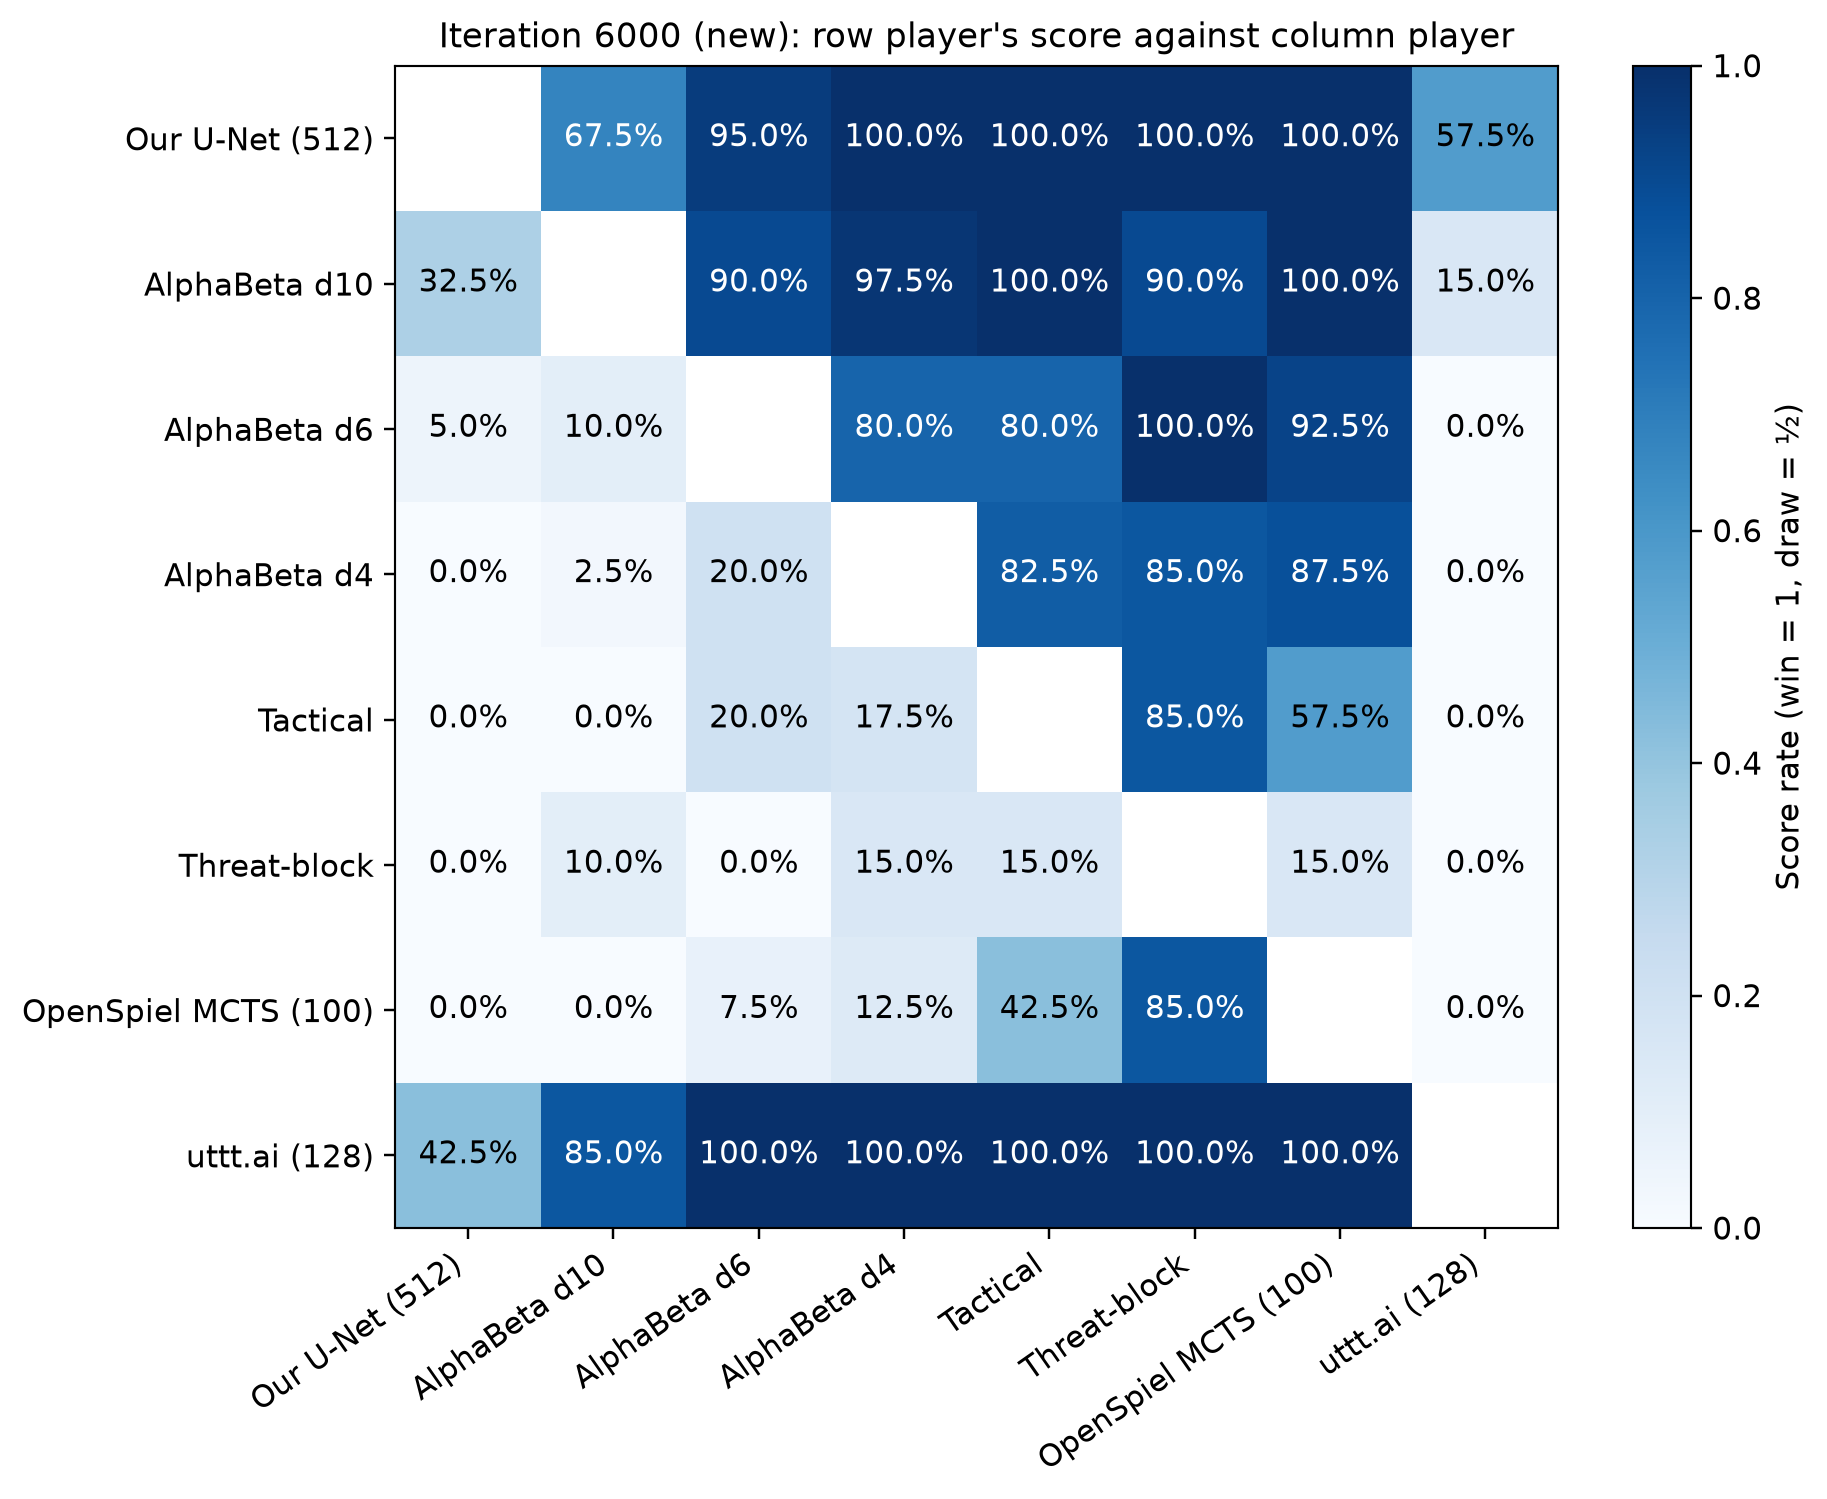
\includegraphics[width=\linewidth]{championship-matrix-iter6000.png}
  \end{minipage}\hfill
  \begin{minipage}[c]{0.60\textwidth}\centering
    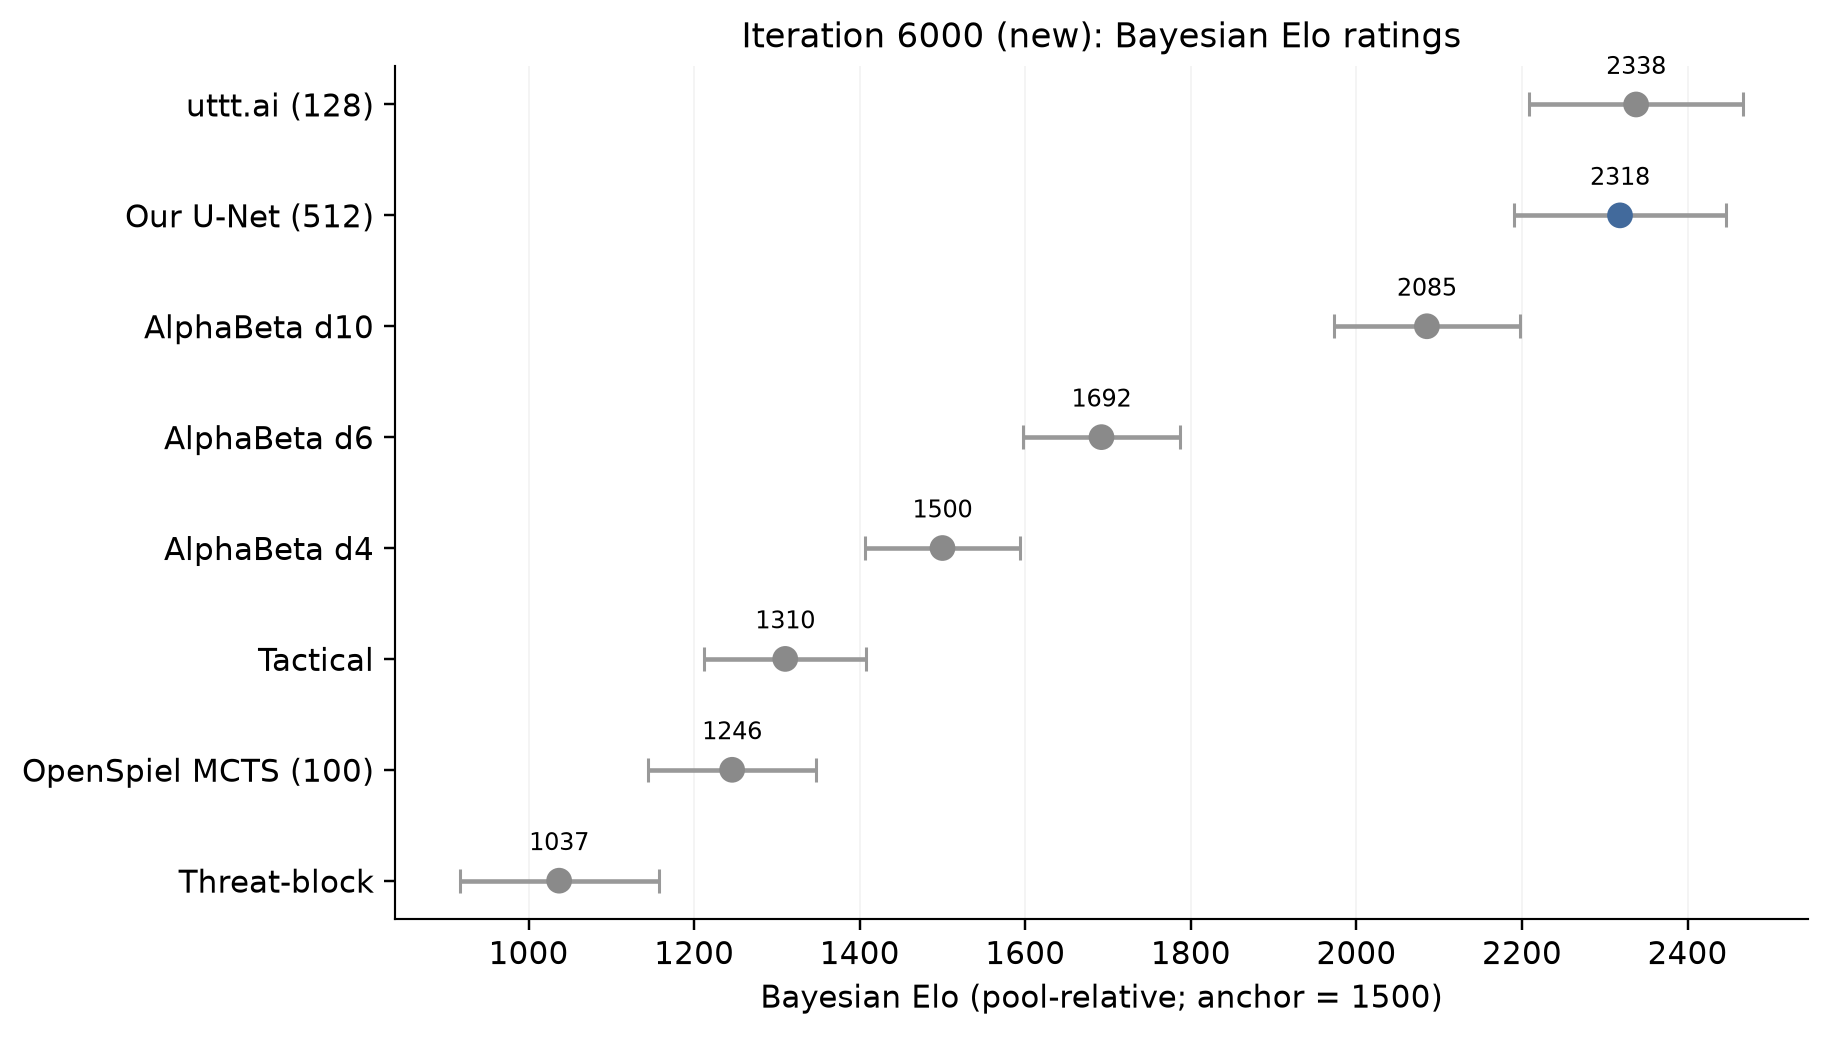
\includegraphics[width=\linewidth]{championship-ratings-iter6000.png}
  \end{minipage}
  \caption{Iteration-6000 championship. Left: round-robin score matrix
  (row player's score against column player). Right: pool-local
  Bayesian-Elo ratings with 95\% CIs, anchored at AlphaBeta d4 $=1500$.}
  \label{fig:champ6000}
\end{figure*}

\section{Evaluation and Results}
\label{sec:results}

\paragraph{Method.}
A checkpoint is evaluated in a round-robin championship. All entrants are
copied and hashed first. Each matchup is played as \emph{opening pairs}: a
seeded random two-ply opening is played twice with the seats swapped, so
first-move advantage cancels. A game scores $1/\tfrac12/0$; a matchup's
score is $(W+\tfrac12D)/(W+D+L)$. Uncertainty is a 95\% bootstrap interval
over opening pairs (10{,}000 resamples), since the two games of a pair are
not independent. Bayesian-Elo ratings anchored at AlphaBeta~d4~$=1500$ are
\emph{pool-local}, not universal. Baselines: C++ alpha--beta at depths 4,
6 and 10 (50-million-node cap), two shallow heuristic bots
(\code{tactical}, \code{threat-block}), OpenSpiel MCTS at 100 rollouts per
decision, and \utttai\ at 128 simulations. The candidate uses 512
simulations and leaf batch 16 (CPU inference for iterations 4193 and 4530,
CUDA for 6000). Budgets are as configured, not equalised for time or
compute.

\paragraph{Results.}
Table~\ref{tab:results} reports three checkpoints. At iteration 4193 (seven
entrants, 20 games per matchup) the agent wins 95--100\% against every
local baseline and scores 35\% against \utttai\ (1--12--7). At iteration
4530 the roster grew to eight entrants with 72 games per matchup (2{,}016
games); the agent finishes second by score (85.8\%, Elo 2201) behind
\utttai\ (91.3\%, Elo 2303) and ahead of depth-10 alpha--beta (71.2\%,
Elo 1960), scoring 41.0\% against \utttai\ (9--41--22). At iteration 6000,
trained with the fixed search and reanalysis, the agent finishes
\emph{first} in a seven-entrant, 420-game round robin (Fig.~\ref{fig:champ6000}):
91.2\% score and Elo 2342 against \utttai's 90.4\% and 2325, with a
5--12--3 head-to-head record (55\%, CI 42.5--70\%). Every other entrant
lost all 20 games to both. The \utttai\ matchup is only ten opening pairs
and its interval includes 50\%: the two engines are now close, not
separated. Against a depth-10 alpha--beta with a $5\times10^{7}$-node cap, iteration
6000 scores 78.5\% over 72 games (48--17--7, CI 70.1--86.8\%), against
71.5\% for iteration 4530 over the same number of games and 67.5\% and
65\% for iterations 1806 and 4193 over 20-game sets. The two 72-game
intervals overlap and use different opening corpora, so this is a
consistent trend, not a measured improvement. A 20-game check of the 4530
checkpoint at 2{,}000 simulations against \utttai\ scored 40\%, far too
small a sample to say anything about search budget.

\paragraph{Search audit.}
Because the gap to \utttai\ was stable, we audited the search with stub
evaluators and known-outcome positions on both backends. Value
perspective, terminal handling, legal moves and Python/C++ parity all
passed. One bug was found: in batched search, once all unexplored branches
were pending, selection kept returning the same terminal leaf, each return
counted against the budget, and the search could exhaust its simulations
before any pending evaluation was applied; with leaf batch 64 in self-play,
endgame targets could be distorted. The fix flushes
the batch after any terminal backup while evaluations are pending; its
footprint is the drop in mean inference batch at iteration 4786 in
Fig.~\ref{fig:training}. The 4193 and 4530 results predate the fix; the
6000 checkpoint was trained from 4786 onward and evaluated with it (native
build \code{63a72ea}). The audit also showed that virtual loss flattens root visit distributions
at large leaf batches (top-move share 0.84 at batch 1 vs.\ 0.06 at batch
64 on the empty board), so self-play trains the policy on softer targets
than a sequential search would give.

% ---------------------------------------------------------------------
\section{Discussion}
\label{sec:discussion}

The pipeline works: an agent trained on one GPU beats a 50-million-node
depth-10 alpha--beta searcher 78.5\% of the time, every shallower baseline
above 90\%, and now holds its own against \utttai. The move from the flat
MLP to \net\ coincided with the first checkpoints that draw rather than
lose against \utttai\ (in the flat-MLP era \utttai\ went 137--2--1 against
the whole field), and the head-to-head score has climbed 27.5\% $\to$ 35\%
$\to$ 41\% $\to$ 55\% across iterations 1806, 4193, 4530 and 6000.

What closed the gap between 4530 and 6000 cannot be attributed: the
search fix, reanalysis, 1{,}470 more iterations and the decaying learning
rate all changed together, and the 6000 head-to-head is ten opening pairs.
The remaining differences from \utttai\ are also open: its network is
about three times larger and was trained on roughly 8~million searched
positions per stage; our policy targets at leaf batch 64 are flattened by
virtual loss; and we regress the value to the game outcome where \utttai\
uses the search value. Each is one controlled experiment away---a larger
\utttai\ match set, a reanalysis on/off comparison, leaf-batch and
value-target ablations---and the launchers exist.

Two limitations apply to every number here. Budgets are configured
simulation counts, not equal wall-clock or compute (the 6000 candidate also
used CUDA inference, and the 4530 championship ran alongside a training
job). And \utttai, OpenSpiel and alpha--beta all appear in the training
population---\utttai\ is the very opponent reanalysis was prioritising---so
these scores do not measure transfer to unseen opponents.

\section{Conclusion}

\sys\ is a complete AlphaZero-style system for Ultimate Tic-Tac-Toe: exact
rules in Python and C++, a two-level policy/value/action-value network,
batched tree search with proofs, a bootstrapped and population-trained
learning loop, and a paired evaluation harness. It dominates every
classical baseline we could construct and, at iteration 6000, finishes
level with the strongest public engine we integrated. The two most useful
findings came from audits rather than training---a learning-rate-driven
value-head collapse and a batched-search starvation bug---and both are now
covered by tests. The next step is controlled experiments---above all a
larger \utttai\ match set---not more features.

\bibliographystyle{IEEEtran}
\bibliography{refs}

\end{document}
